\documentclass[11pt,a4paper]{article}
\usepackage[top=21mm,bottom=20mm,left=18mm,right=18mm,headheight=13pt,headsep=7mm,footskip=10mm]{geometry}
\usepackage{fontspec}
\setmainfont{texgyreheros-regular.otf}[BoldFont=texgyreheros-bold.otf,ItalicFont=texgyreheros-italic.otf,BoldItalicFont=texgyreheros-bolditalic.otf]
\setsansfont{texgyreheros-regular.otf}[BoldFont=texgyreheros-bold.otf]
\setmonofont{texgyrecursor-regular.otf}[Scale=0.9]
\usepackage[british]{babel}
\usepackage[table]{xcolor}
\definecolor{brand}{HTML}{176D5B}
\definecolor{ink}{HTML}{202E35}
\definecolor{muted}{HTML}{68777E}
\definecolor{pale}{HTML}{E9F3EE}
\definecolor{paper}{HTML}{F5F7F8}
\definecolor{line}{HTML}{E0E7E6}
\definecolor{amber}{HTML}{88652B}
\definecolor{cream}{HTML}{F8F0DD}
\usepackage{graphicx,booktabs,tabularx,array,microtype,ragged2e}
\usepackage{tikz}
\usetikzlibrary{arrows.meta,positioning,calc,svg.path}
\usepackage[most]{tcolorbox}
\usepackage{fancyhdr,enumitem,hyperref}
\hypersetup{colorlinks=true,linkcolor=brand,urlcolor=brand,pdftitle={SchedU — User manual},pdfauthor={SchedU},pdfsubject={Guidance for students, instructors and administrators},pdfkeywords={SchedU, tutorials, booking, user manual},pdflang={en-GB},bookmarksopen=true}
\graphicspath{{assets/}}
\color{ink}
\linespread{1.055}
\setlength{\parindent}{0pt}
\setlength{\parskip}{6pt}
\setlength{\tabcolsep}{7pt}
\renewcommand{\arraystretch}{1.24}
\raggedbottom
\emergencystretch=2em
\hyphenation{progress select selected review offer}
\setlist[enumerate]{leftmargin=5mm,itemsep=4pt,topsep=3pt,label=\textcolor{brand}{\arabic*.}}
\newcolumntype{L}[1]{>{\raggedright\arraybackslash}p{#1}}
\newcolumntype{Y}{>{\raggedright\arraybackslash}X}
\pagestyle{fancy}
\fancyhf{}
\fancyhead[L]{\small\bfseries\textcolor{brand}{SchedU}\ \textcolor{muted}{/ User manual}}
\fancyhead[R]{\small\textcolor{muted}{\nouppercase{\leftmark}}}
\fancyfoot[L]{\footnotesize\textcolor{muted}{October 2026}}
\fancyfoot[R]{\footnotesize\textcolor{brand}{\thepage}}
\renewcommand{\headrulewidth}{0pt}
\newcommand{\eyebrow}[1]{{\small\bfseries\textcolor{brand}{\MakeUppercase{#1}}}\par}
\newcommand{\manualpage}[3]{\clearpage\phantomsection\label{#3}\pdfbookmark[0]{#2}{bm-#3}\markboth{#1}{}\eyebrow{#1}\vspace{1mm}{\fontsize{25}{29}\selectfont\bfseries #2\par}\vspace{3mm}}
\newcommand{\subhead}[1]{\par\vspace{2mm}{\large\bfseries #1\par}\vspace{0.5mm}}
\newcommand{\ui}[1]{\textbf{#1}}
\newcommand{\smallcaption}[1]{{\fontsize{9}{12}\selectfont\color{muted}#1\par}}
\newcommand{\shot}[3][width=\linewidth]{\par\vspace{2mm}{\centering\includegraphics[#1]{#2}\par}\vspace{1mm}\smallcaption{#3}\vspace{2mm}}
\newtcolorbox{note}[1][]{colback=pale,colframe=pale,boxrule=0pt,arc=2mm,left=4mm,right=4mm,top=3mm,bottom=3mm,before skip=7pt,after skip=7pt,#1}
\newcommand{\tocrow}[2]{\hyperref[#2]{#1} & \textcolor{brand}{\pageref{#2}}\\}
\newcommand{\logo}[1]{\resizebox{#1}{!}{
\begin{tikzpicture}[x=1pt,y=1pt,yscale=-1]
\path[use as bounding box] (0,0) rectangle (320,320);
\path[fill=brand] svg{M66 34H49C29 34 14 49 14 70V264C14 285 29 300 49 300H172L154 278H49C41 278 36 272 36 264V107H295V70C295 49 280 34 259 34H241V56H258C267 56 273 62 273 71V86H36V71C36 62 42 56 50 56H66Z};
\fill[brand,rounded corners=6pt] (66,18) rectangle (89,70);
\fill[brand,rounded corners=6pt] (219,18) rectangle (242,70);
\fill[brand,rounded corners=6pt] (115,32) rectangle (141,58);
\fill[brand,rounded corners=6pt] (167,32) rectangle (193,58);
\path[fill=brand] svg{M166 134H220V155H204V263L219 278H257L272 263V155H255V134H311V155H295V268Q295 272 292 275L271 296Q267 300 262 300H216Q211 300 207 296L186 275Q182 271 182 266V155H166Z};
\end{tikzpicture}}}
\begin{document}
\thispagestyle{empty}
\pdfbookmark[0]{SchedU user manual}{cover}
\begin{tikzpicture}[remember picture,overlay]
\fill[pale] (current page.north west) rectangle ([yshift=-102mm]current page.north east);
\fill[brand] ([xshift=18mm,yshift=-102mm]current page.north west) rectangle ([xshift=60mm,yshift=-104mm]current page.north west);
\end{tikzpicture}
\vspace*{4mm}
\logo{23mm}\hspace{4mm}{\fontsize{39}{43}\selectfont\bfseries Sched\textcolor{brand}{U}}
\vspace{13mm}

{\fontsize{37}{41}\selectfont\bfseries User manual\par}
\vspace{3mm}
{\Large Face-to-face tutorial booking\par}
\vspace{25mm}

{\large For students, instructors and administrators\par}
\vspace{4mm}
SchedU brings tutorial availability, bookings and feedback into one workspace. Students reserve a time slot; instructors record attendance and feedback; administrators manage accounts and the timetable.

This manual explains the everyday tasks for each role. System administration and server maintenance are outside its scope.

\vspace{10mm}
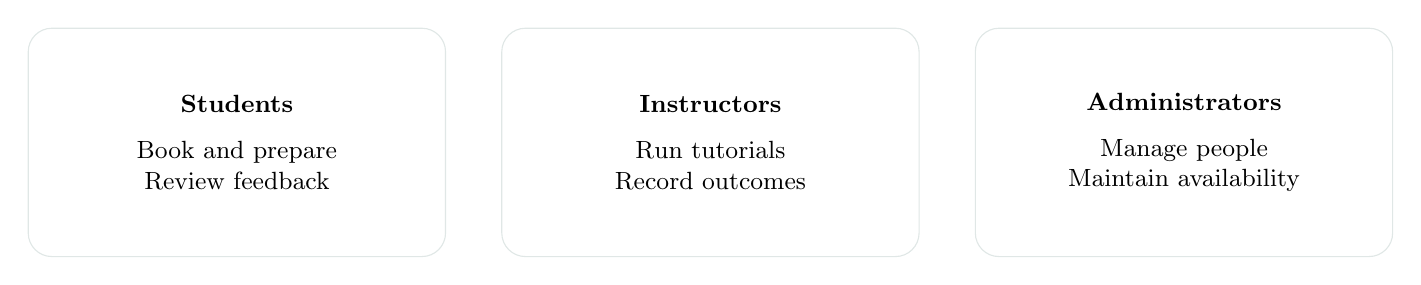
\begin{tikzpicture}[node distance=7mm, every node/.style={font=\small}, card/.style={draw=line,rounded corners=3mm,minimum width=53mm,minimum height=29mm,align=center,fill=white}]
\node[card] (s) {\textbf{Students}\\[2mm]Book and prepare\\Review feedback};
\node[card,right=7mm of s] (i) {\textbf{Instructors}\\[2mm]Run tutorials\\Record outcomes};
\node[card,right=7mm of i] (a) {\textbf{Administrators}\\[2mm]Manage people\\Maintain availability};
\end{tikzpicture}
\vfill
\smallcaption{Edition 1 · October 2026}

\manualpage{Using this manual}{Find the guidance for your role}{contents}
Read the shared guidance first, then the pages for your assigned role. In SchedU, a teacher’s role is called \ui{Instructor}. Your role determines which pages and actions appear.

\begin{tabularx}{\linewidth}{@{}Yr@{}}
\toprule
\textbf{Shared guidance} & \textbf{Page}\\
\tocrow{Sign in and choose your preferences}{signin}
\tocrow{Check your profile and dashboard}{profile}
\addlinespace[2mm]
\textbf{Students} & \\
\tocrow{Choose a tutorial}{book}
\tocrow{Confirm, track or cancel a booking}{manage}
\tocrow{Read your feedback}{feedback}
\addlinespace[2mm]
\textbf{Instructors} & \\
\tocrow{Prepare for and run a tutorial}{instructor}
\tocrow{Record attendance and feedback}{evaluate}
\addlinespace[2mm]
\textbf{Administrators} & \\
\tocrow{Manage bookings and exceptions}{adminbookings}
\tocrow{Manage people and accounts}{people}
\tocrow{Import a roster}{roster}
\tocrow{Use account filters and batch actions}{bulk}
\tocrow{Read the availability calendar}{calendar}
\tocrow{Set up recurring teaching windows}{windows}
\tocrow{Import a timetable and adjust individual slots}{timetable}
\tocrow{Remove sessions across the semester}{remove}
\addlinespace[2mm]
\tocrow{Resolve common problems}{help}
\bottomrule
\end{tabularx}

\subhead{How the work fits together}
\begin{center}
\begin{tikzpicture}[every node/.style={font=\small,align=center},box/.style={draw=line,fill=paper,rounded corners=2mm,minimum height=13mm,text width=46mm},arr/.style={-Latex,thick,brand}]
\node[box] (a) at (0,0) {\textbf{Administrator}\\Publishes availability};
\node[box] (s) at (5.9,0) {\textbf{Student}\\Reserves a time slot};
\node[box] (i) at (11.8,0) {\textbf{Instructor}\\Records the outcome};
\node[box,fill=pale,text width=92mm] (shared) at (5.9,-2.1) {\textbf{Shared SchedU records}\\Timetable · booking status · attendance · feedback};
\draw[arr] (a)--(s);\draw[arr] (s)--(i);
\draw[arr] (a.south)|-(shared.west);
\draw[arr] (s.south)--(shared.north);
\draw[arr] (i.south)|-(shared.east);
\end{tikzpicture}
\end{center}
\smallcaption{The tutorial itself takes place in the listed classroom. Students see their own records; instructors work with assigned sessions; administrators manage the wider schedule.}

\manualpage{Everyone}{Sign in and choose your preferences}{signin}
Open the SchedU address supplied by your institution. Enter your \ui{Institutional ID} and password, then select \ui{Sign in}. Use the account issued by an administrator; there is no self-registration step.

\begin{minipage}[t]{.46\linewidth}
\shot[width=\linewidth]{sign-in.png}{The sign-in form uses your student or staff ID.}
\end{minipage}\hfill
\begin{minipage}[t]{.49\linewidth}
\shot[width=\linewidth]{first-login.png}{At first sign-in, you may change or keep the issued password.}
\end{minipage}

\subhead{Your first sign-in}
To change the issued password, enter it under \ui{Current password}, enter a new password of 8–128 characters twice, and select \ui{Update password}. The alternative, \ui{Keep my initial password}, dismisses the prompt without changing it. You can change your password later from \ui{My profile}.

If you have forgotten your password, contact an administrator. An administrator can issue a replacement; the app does not offer an email recovery link.

\subhead{Language and appearance}
The language control at the top of the page switches between English and Simplified Chinese. The \ui{Theme} menu offers \ui{Light}, \ui{Dark} and \ui{System}. System follows the browser or operating system’s appearance setting. It does not use the tutorial start time to decide when to switch.

Preferences are remembered on the device. Changing language or theme does not change your bookings. Use \ui{Sign out} beside your account details when you finish on a shared computer.

\begin{note}
\textbf{Time zone}\par
Meeting dates and times always use China Standard Time (UTC+8), including when you open SchedU from another time zone.
\end{note}

\manualpage{Everyone}{Check your profile and dashboard}{profile}
Open \ui{My profile} and check your details before using the booking service. Your institutional ID is displayed for reference and cannot be edited here. Ask an administrator if it is incorrect.

\shot[width=.91\linewidth]{profile.png}{A completed first-year student profile. The phone number is optional.}

\begin{tabularx}{\linewidth}{@{}L{40mm}Y@{}}
\toprule
\textbf{Field} & \textbf{What to enter}\\
\midrule
Entry year & Your student entry year, or the year you joined the organisation as a member of staff. The Chinese label uses a neutral term for joining.\\
Chinese / English name & Use the names by which staff can identify you. Both are required for students; staff must supply a Chinese name.\\
Administrative class & Required for every student. Choose the class from the list.\\
Teaching class & Required when the student entry year matches the current calendar year in China. Optional for earlier cohorts.\\
Phone number & Optional. If supplied, it must use a valid phone-number format.\\
\bottomrule
\end{tabularx}

Select \ui{Save profile} after making changes. Class lists are defined by the institution. If the correct class is missing, contact an administrator rather than choosing an unrelated class.

\subhead{Use Overview to decide what to do next}
\ui{Overview} summarises your activity and upcoming tutorials. Students can check active bookings, attendance and feedback, then open \ui{Book a tutorial}, \ui{My bookings} or \ui{My feedback}. Instructors see their teaching activity and sessions; administrators see an institution-wide summary.

The navigation changes with your assigned role. You cannot grant yourself another role from your profile.

\manualpage{Students}{Choose a tutorial}{book}
Select \ui{Book a tutorial}. Choose a date, then open \ui{Available time slot}. Each option shows the date, meeting time, classroom and remaining seats. Use the week arrows to browse further ahead within the institution’s booking period.

\shot[width=\linewidth]{book-tutorial.png}{A Tuesday booking for 18:30–18:40. Two instructors are on duty, and two seats remain before submission.}

You reserve a time slot, not a named instructor. You may meet any instructor listed as on duty. Check that you can reach the classroom for the start time, then add a brief question or topic if useful. The topic is optional.

\ui{Save draft} keeps an unfinished booking under \ui{My bookings → Drafts}. A draft does not reserve a seat. Open its details and select \ui{Continue draft} to return to the form, or \ui{Delete draft} to remove it without a cancellation pause.

Select \ui{Review booking} when you are ready. Your student profile must be complete before you can submit. The demonstration allows one active booking at a time and shows availability for the next 28 days; your institution can change these limits.

\manualpage{Students}{Confirm, track or cancel a booking}{manage}
Review the date, time, classroom and cancellation rule, then select \ui{Confirm booking}. A slot with an assigned instructor is approved automatically. An unstaffed slot stays \ui{Submitted} until a member of staff approves it.

\begin{minipage}[t]{.53\linewidth}
\shot[width=\linewidth]{review-booking.png}{Submission confirms the selected time and its cancellation policy.}
\end{minipage}\hfill
\begin{minipage}[t]{.43\linewidth}\RaggedRight
\shot[width=\linewidth]{cancel-booking.png}{Choose \ui{Keep booking} to leave the reservation in place.}
\smallcaption{The pause shown here is two weeks. Always read the period displayed by your institution.}
\end{minipage}

Open \ui{My bookings → Upcoming \& active} to check the result. \ui{View details} shows the classroom, instructor pool, topic and status history. Drafts and past records have separate tabs.

\subhead{The booking’s progress}
\begin{center}
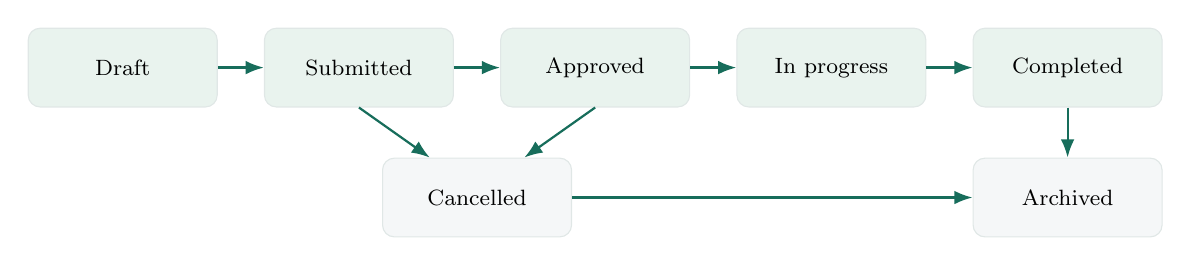
\begin{tikzpicture}[every node/.style={font=\footnotesize,align=center},box/.style={draw=line,fill=pale,rounded corners=1.5mm,minimum height=10mm,minimum width=24mm},arr/.style={-Latex,brand,thick}]
\node[box] (d) at (0,0) {Draft};
\node[box] (s) at (3,0) {Submitted};
\node[box] (a) at (6,0) {Approved};
\node[box] (i) at (9,0) {In progress};
\node[box] (c) at (12,0) {Completed};
\node[box,fill=paper] (x) at (4.5,-1.65) {Cancelled};
\node[box,fill=paper] (r) at (12,-1.65) {Archived};
\draw[arr] (d)--(s);\draw[arr] (s)--(a);\draw[arr] (a)--(i);\draw[arr] (i)--(c);
\draw[arr] (s.south)--([xshift=-6mm]x.north);\draw[arr] (a.south)--([xshift=6mm]x.north);
\draw[arr] (c)--(r);\draw[arr] (x)--(r);
\end{tikzpicture}
\end{center}
\smallcaption{Automatic approval moves straight to Approved. Staff may save feedback from Approved once the tutorial has started, without first selecting In progress. Archiving retains the record.}

\subhead{If you need to cancel or change the time}
A student can cancel a submitted or approved booking before its start time. Open its details, select \ui{Cancel booking} and read the confirmation. Confirming cancellation pauses new bookings from that moment for the displayed period. It does not automatically cancel other existing bookings.

\begin{note}[colback=cream,colframe=cream]
There is no direct rescheduling action. If you need a different time, contact an administrator before cancelling: cancelling the booking yourself starts the booking pause. A cancellation made by authorised staff does not apply this student penalty.
\end{note}

\manualpage{Students}{Read your feedback}{feedback}
After the tutorial, open \ui{My feedback}. Each card shows the meeting date, evaluation mark, description and any written advice. Completed feedback remains available when the meeting is archived.

\shot[width=\linewidth]{student-feedback.png}{Two completed tutorials for the same student. Written feedback identifies what to practise next.}

\subhead{Understanding the evaluation}
The mark is one of the institution’s configured evaluation options. It is not a percentage or a score out of 100 unless your institution explicitly uses it that way. The demonstration uses these standard options.

\begin{tabularx}{\linewidth}{@{}L{20mm}Y@{}}
\toprule
\textbf{Mark} & \textbf{Meaning}\\
\midrule
0 & Absent.\\
30 & Attended with poor performance.\\
40 & Completed with satisfactory performance.\\
70 & Completed with excellent performance.\\
\bottomrule
\end{tabularx}

Read the written comment alongside the mark. Use it to identify a specific exercise, explanation or question to prepare for your next tutorial. If there is no written comment, the evaluation still records the outcome.

\subhead{Before your next meeting}
Check \ui{My bookings} for the confirmed time and room. Bring the work or question you described when booking. Arrive in time for the short appointment; the gap after it is reserved for the teaching schedule and is not additional tutorial time.

If feedback or attendance appears incorrect, contact the instructor or an administrator with the meeting date and time. Students cannot edit evaluation records.

\begin{note}
\textbf{No feedback yet?}\par
An approved or in-progress booking has not been completed. Check its status first. Ask the instructor if the tutorial has finished but the feedback has not appeared.
\end{note}

\manualpage{Instructors}{Prepare for and run a tutorial}{instructor}
Use \ui{Overview} to review your activity, then open \ui{My sessions} for the bookings assigned to your instructor pool. A student has reserved a place in the time slot and may meet any instructor on duty.

\begin{minipage}[t]{.43\linewidth}\RaggedRight
\subhead{Before the appointment}
Open \ui{View details} to check the student’s name, institutional ID, class and topic. Confirm the room and scheduled time.

If a booking is \ui{Submitted} and falls within your responsibility, \ui{Approve} confirms it before the start time. If it is outside your assigned sessions, ask an administrator to handle it.

\subhead{At the appointment}
For an approved booking, \ui{Start session} becomes available at the scheduled start time. This changes its status to \ui{In progress}.

After the tutorial, use \ui{Record feedback}. It is also possible to record feedback directly from an approved booking once its start time has passed.

When several instructors share a slot, coordinate who will record the outcome. Check the current status before acting.
\end{minipage}\hfill
\begin{minipage}[t]{.53\linewidth}
\shot[width=\linewidth]{instructor-details.png}{An in-progress tutorial, with the student’s details, topic and status history.}
\end{minipage}

\subhead{Cancellations and changes}
Instructor cancellation is disabled by default. If your institution enables it, \ui{Cancel booking} appears for submitted or approved bookings that you manage. An instructor cancellation does not pause the student’s future booking rights.

If the action is unavailable, ask an administrator to manage the change. In-progress and completed bookings cannot be cancelled through this action. Arrange any necessary timetable change through an administrator.

\manualpage{Instructors}{Record attendance and feedback}{evaluate}
Open a started tutorial’s details and select \ui{Record feedback}. Choose the appropriate \ui{Attendance \& performance} option, add feedback for the student, then select \ui{Complete \& save feedback}.

\shot[width=.65\linewidth]{record-feedback.png}{The selected evaluation and written comment are saved together. The student can read the comment.}

\subhead{Record the outcome accurately}
Use the institution’s evaluation descriptions, rather than treating the numerical mark as a free-entry score. The default options are shown on page~\pageref{feedback}. Give a brief account of the student’s work and a concrete next step when written feedback would help.

An attended tutorial can be completed from \ui{Approved} or \ui{In progress} after the scheduled start time. The \ui{0 · Absent} option cannot be saved before the scheduled end time. Wait until the whole appointment has elapsed before recording a non-attendance.

\subhead{After saving}
Saving the evaluation changes the booking to \ui{Completed}. The student can read it under \ui{My feedback}; you can review completed outcomes under \ui{Feedback}. The booking no longer counts towards the student’s active-booking limit.

Open the details of a completed or cancelled booking and select \ui{Archive} when it should be retained as a past record. Archiving does not delete the booking, its history or its feedback.

\begin{note}
Check the mark and wording before saving. The current interface does not offer a general edit action for a completed evaluation. If a correction is needed, report the booking details to an administrator.
\end{note}

\manualpage{Administrators}{Manage bookings and exceptions}{adminbookings}
Open \ui{All meetings} to review bookings across the institution. \ui{Upcoming \& active} contains submitted, approved and in-progress bookings; \ui{History} contains past outcomes. Select \ui{View details} to inspect a meeting and its status history.

\shot[width=.96\linewidth]{admin-meetings.png}{An administrator’s view of active bookings. Each record identifies the student, time, room and current status.}

\subhead{Approve a pending booking}
For a \ui{Submitted} booking, confirm that the tutorial can be staffed and then select \ui{Approve} before its scheduled start. Staffed slots are normally approved automatically when students book them. An administrator can act across the schedule, including bookings outside a particular instructor’s pool.

\subhead{Handle a cancellation or timetable change}
Open the submitted or approved booking and select \ui{Cancel booking}. Review the confirmation before proceeding. A management cancellation does not impose the student booking pause. Inform the student about the change through your institution’s usual channel.

There is no direct move-to-another-slot action. Where a schedule change affects existing bookings, arrange it with the students, resolve the active reservations and then update availability. In-progress and completed bookings cannot be cancelled through the cancellation action.

\subhead{Complete or archive a record}
Administrators have the same \ui{Start session}, \ui{Record feedback} and \ui{Archive} controls described on pages~\pageref{instructor}–\pageref{evaluate}. The same start-time and absence checks apply. When completing a record on an instructor’s behalf, confirm the attendance and evaluation with the instructor first.

Archiving a completed or cancelled booking preserves its history and feedback. It does not remove account dependencies or make a linked account eligible for ordinary deletion.

\manualpage{Administrators}{Manage people and accounts}{people}
\ui{People \& rosters} lists the accounts in SchedU. Search by institutional ID, name or administrative class. A missing teaching class is displayed as \ui{Unassigned Teaching Class}; it is allowed for students from earlier entry cohorts.

\shot[width=\linewidth]{people-rosters.png}{The account list includes role controls, profile editing and account actions. This view shows the first two rows.}
\shot[width=\linewidth]{roster-pagination.png}{There are 50 accounts per page. Use numbered pages, First, Last or Go to page to move through the roster.}

\subhead{Issue, update and remove accounts}
\ui{Issue account} creates a student or instructor account with an institutional ID and names. A random initial password is then displayed. Download the credentials and give each user their own details privately. A student must complete any missing profile fields before submitting a booking.

Use \ui{Edit} on an account row to correct personal details. The role menu changes a student to an instructor, or an instructor to a student. Existing active bookings or teaching assignments may prevent a role change. Changing a role ends that account’s current sessions.

\ui{Reset password} issues a replacement and ends the account’s current sessions. \ui{Delete} removes an unused account; meeting records or instructor assignments prevent ordinary deletion. Resolve the reported dependency or seek help from the system administrator.

\smallcaption{Ordinary administrators manage students and instructors. Administrator privileges, global configuration and full-system maintenance belong to the system administrator.}

\manualpage{Administrators}{Import a roster}{roster}
Use \ui{CSV template} on \ui{People \& rosters} as the starting point. Save the completed file as a UTF-8 CSV so that Chinese names and class labels are preserved. Keep institutional IDs as text in a spreadsheet, particularly if they contain leading zeroes.

\begin{tabularx}{\linewidth}{@{}L{36mm}Y@{}}
\toprule
\textbf{CSV column} & \textbf{Content}\\
\midrule
\texttt{id} & Unique institutional ID. Existing IDs cannot be overwritten by a roster import.\\
\texttt{role} & \texttt{student} or \texttt{instructor}. A blank value means student.\\
\texttt{grade} & Entry or joining year, for example \texttt{2026}.\\
\texttt{adminClass} & Exact administrative class label from the configured list; required for students.\\
\texttt{teachingClass} & Exact teaching class label. Required for the current-year student cohort; otherwise it may be blank.\\
\texttt{chineseName} & Chinese name.\\
\texttt{englishName} & English name; required for students.\\
\texttt{phone} & Optional. Leave the cell blank if no number is supplied.\\
\bottomrule
\end{tabularx}

Select \ui{Import roster} and choose the file. Review the names, classes and validation results before selecting \ui{Import \& issue passwords}. Correct duplicate IDs or invalid fields in the source file and import again. If validation fails, the import creates no accounts.

\shot[width=.93\linewidth]{roster-import.png}{A two-account preview: the earlier-cohort student has no teaching class.}

The preview displays the first 50 rows, but a successful import processes every row. Roster imports have no account-count limit; the request must still fit within the 20 MB size limit. The separate limit of 100 selected accounts applies to batch actions, not imports.

Download the generated credentials while they are displayed. Passwords are shown once. Do not distribute the full credentials file to students; provide only the details for each person’s account.

\manualpage{Administrators}{Use account filters and batch actions}{bulk}
The status controls above the roster show \ui{All accounts}, \ui{Booking paused}, \ui{Active} or \ui{First login pending}. They describe account status, not the status of a particular tutorial. Changing the status filter clears your selection.

\shot[width=\linewidth]{paused-accounts.png}{Filter to Booking paused, select the required student and choose Lift booking pause.}

\subhead{Lift a booking pause}
Select \ui{Booking paused} and tick the students whose restrictions should be lifted. Choose \ui{Lift booking pause} under \ui{Bulk action}, then select \ui{Apply to selected}. Review the confirmation and apply it to the intended accounts.

Only selected students who currently have a booking pause are eligible. Lifting the pause restores their ability to make new bookings, subject to the other booking rules. It preserves passwords, signed-in sessions and meeting history.

\subhead{Other batch actions}
The same selection controls support password resets, student/instructor role changes and deletion. Select up to 100 accounts, choose the action and review the confirmation before applying it. Validation applies to the whole selection: a failure leaves the selection unchanged.

Password resets issue new credentials and end the affected accounts’ sessions. Role changes must satisfy the same booking and assignment checks as an individual change. Deletion remains unavailable for accounts with meeting records or teaching assignments.

\begin{note}
\textbf{Check the selection before confirming}\par
Searches and status filters help narrow the list, but the operation applies to the selected accounts. Read the selection count and confirmation, especially when moving between roster pages.
\end{note}

\manualpage{Administrators}{Read the availability calendar}{calendar}
\ui{Availability} opens a 28-day view. Use \ui{Previous 4 weeks}, \ui{Next 4 weeks}, \ui{Show dates from} or \ui{Semester start} to view another period. Select a date to manage its individual time slots below the calendar.
\shot[width=.88\linewidth]{availability-calendar.png}{Rooms, instructors and remaining seats are shown for each date. Date off means the day is closed. Administrators can view dates beyond the student booking period. The displayed time range spans the generated slots and can be shorter than the teaching window.}

\manualpage{Administrators}{Set up recurring teaching windows}{windows}
A teaching window defines a weekly period, room, instructor pool and capacity. SchedU divides that period into individual appointments. The system administrator must first configure semester dates, classrooms and the meeting/break lengths.

\begin{minipage}[t]{.46\linewidth}\RaggedRight
\subhead{Create a weekly series}
In \ui{Availability}, select \ui{Add teaching window}. Choose the weekday, starting teaching week, time range and classroom. Set \ui{Students per slot}, tick the instructors on duty, and leave \ui{Offer slots in this window} selected to publish it.

Check the date preview, then select \ui{Save teaching window}. Assigned instructors enable automatic booking approval. Capacity is the number of students allowed in each slot; it is a separate setting from the number of instructors.

\subhead{Set the end of the series}
Leave \ui{Repeat for (weeks)} blank to continue through the semester’s end. Enter a number to stop earlier. A longer count is clipped at the final semester date.

Teaching weeks run Monday to Sunday. Week 1 contains the semester start date. No dates are generated before the semester starts or after it ends. Dates off do not extend the series.

\subhead{Maintain the series}
Expand \ui{Weekly teaching windows} to edit an existing window. Clear its offer checkbox to pause it, or use \ui{Remove} to remove it. Active bookings protect their slots from conflicting changes.
\end{minipage}\hfill
\begin{minipage}[t]{.51\linewidth}
\shot[width=\linewidth]{teaching-window.png}{Example: week 5 through semester end gives 15 Tuesdays, from 6 October to 12 January, before any dates off.}
\end{minipage}

\manualpage{Administrators}{Import a timetable and adjust slots}{timetable}
For several recurring windows, use \ui{Import weekly timetable} under \ui{Weekly teaching windows}. Download the template, fill one row per window, select \ui{Choose CSV}, review the preview and confirm the import. Import adds windows to the existing timetable.

\begin{tabularx}{\linewidth}{@{}L{39mm}Y@{}}
\toprule
\textbf{CSV column} & \textbf{Example and rule}\\
\midrule
\texttt{day} & \texttt{Wednesday}; weekday names are accepted.\\
\texttt{instructors} & \texttt{STAFF1001;STAFF1002}; use existing account IDs, separated by semicolons.\\
\texttt{start}, \texttt{end} & \texttt{18:30}, \texttt{20:05}; use 24-hour times.\\
\texttt{location} & Exact classroom label, such as Engineering Building · Room 302.\\
\texttt{capacity} & \texttt{2}; students allowed in each slot.\\
\texttt{startWeek}, \texttt{repeatWeeks} & \texttt{5}, \texttt{12}; optional. Blank means week 1 through semester end.\\
\bottomrule
\end{tabularx}

An unknown instructor, unconfigured classroom or overlapping instructor assignment prevents the import. Correct the source file and review it again. Semester dates must already be set.

\subhead{How a window becomes appointments}
\begin{center}

\begin{tikzpicture}[x=1mm,y=1mm,every node/.style={font=\footnotesize,align=center}]
\fill[pale,rounded corners=1mm] (0,0) rectangle (46,16);
\fill[paper] (47,0) rectangle (69,16);
\fill[pale,rounded corners=1mm] (70,0) rectangle (116,16);
\fill[paper] (117,0) rectangle (139,16);
\node at (23,8) {Tutorial\\18:30–18:40};
\node at (58,8) {Break\\5 min};
\node at (93,8) {Tutorial\\18:45–18:55};
\node at (128,8) {Break\\5 min};
\node[text=brand] at (153,8) {Continues\\every 15 min};
\draw[-Latex,brand] (0,-4)--(166,-4);
\end{tikzpicture}
\end{center}
\smallcaption{With ten-minute tutorials and five-minute breaks, the final appointment in an 18:30–20:05 window is 19:45–19:55. A 20:00 start is excluded because it would end after the window.}

\subhead{Change one occurrence}
In the calendar, select the date and find \ui{Individual time slots}. Use \ui{Edit} to adjust a single occurrence, \ui{Delete} to close or remove it, or \ui{Add time slot} for a one-off appointment. Select the configured classroom and instructor pool, then save.

A deleted recurring occurrence stays closed on that date; the weekly series remains. Reopen it through the individual slot controls if needed. A deleted one-off slot is removed. Active bookings must be resolved before their slot is changed.

\ui{Dates off} closes whole days. Enter one date per line in \texttt{YYYY-MM-DD} format and select \ui{Save dates off}. Resolve active bookings on those dates first.

\manualpage{Administrators}{Remove sessions across the semester}{remove}
Open \ui{Availability → All semester sessions} to find sessions beyond the four-week calendar. Set the date range and, if useful, filter by weekday, classroom, instructor or teaching window before selecting rows.

\shot[width=.92\linewidth]{semester-sessions.png}{An excerpt of six selected Tuesday sessions. Select all matching sessions includes every matching page.}

\begin{minipage}[t]{.47\linewidth}\RaggedRight
Select individual rows, \ui{Select this page}, or \ui{Select all … matching sessions}. Choose \ui{Review removal} and check the counts before confirming.

Sessions with submitted, approved or in-progress bookings are kept. The app removes only sessions without active bookings, and checks again when you confirm.
\end{minipage}\hfill
\begin{minipage}[t]{.49\linewidth}
\shot[width=\linewidth]{remove-sessions.png}{This example keeps two booked sessions and removes four unbooked sessions.}
\end{minipage}

Removed recurring occurrences stay closed; removed one-off slots disappear. Weekly teaching-window definitions and all booking, history and feedback records remain. Students receive no cancellation pause from this operation.

If the schedule changes before confirmation, review the selection again. This operation clears availability; it is not a full-system data reset.

\manualpage{Everyone}{Resolve common problems}{help}
\begin{tabularx}{\linewidth}{@{}L{48mm}Y@{}}
\toprule
\textbf{What you see} & \textbf{What to check or do}\\
\midrule
Cannot sign in & Check the institutional ID and password supplied to you. Contact an administrator for a password reset if needed.\\
\addlinespace
Review booking is unavailable & Select a slot, complete your profile and check whether you have reached the active-booking limit or have a booking pause.\\
\addlinespace
No suitable time slots & Try another date within the booking period. Slots may be full, closed, past their start time or not yet published. Ask an administrator about availability.\\
\addlinespace
Booking is still Submitted & The slot had no assigned instructor when submitted. Ask an administrator to confirm the staffing and approval.\\
\addlinespace
Booking paused & Check the end date shown in the app. An administrator may lift the restriction where appropriate. Your existing records remain available.\\
\addlinespace
Cancel booking is missing & Students can cancel only submitted or approved bookings before the start. Instructors need the cancellation setting enabled and responsibility for the booking.\\
\addlinespace
Absent cannot be saved & Wait until the tutorial’s scheduled end time before recording a mark of zero.\\
\addlinespace
Class or room is missing & Ask an administrator to check the institution’s list. An ordinary administrator must refer changes to those lists to the system administrator.\\
\addlinespace
Roster import fails & Check duplicate IDs, required names, entry years and exact class labels. Save as UTF-8 CSV and review the errors. No rows are imported on validation failure.\\
\addlinespace
Schedule change or deletion is blocked & Look for active bookings and instructor assignments. Batch session removal keeps booked sessions automatically. Ordinary account deletion preserves linked meeting records by refusing the deletion.\\
\bottomrule
\end{tabularx}

\subhead{Ask the right person}
Students should contact an instructor about the tutorial or its feedback, and an administrator about account details, access or booking arrangements. Instructors should refer timetable changes and account issues to an administrator.

Ordinary administrators manage meetings, schedules and student/instructor accounts. The system administrator controls global booking rules, semester dates, class and classroom lists, evaluation options, administrator privileges and system maintenance.

When reporting a problem, include the institutional ID, meeting date and time, the action attempted and any displayed error. Do not send a password. A screenshot may help, but avoid sharing other people’s personal information.
\end{document}
